%~ \subsection{Descripción del problema.}
%~
%~ \vspace*{0.3cm}
%~
%~ En este problema, debemos encontrar una \textbf{secuencia de vuelos que
%~ permita}, dada una ciudad de origen, otra de destino y un listado de vuelos,
%~ \textbf{viajar del origen al destino, llegando lo más temprano posible}.
%~
%~ Esta secuencia \textbf{debe comenzar con un vuelo que parta de la ciudad
%~ origen}. Luego, \textbf{cada vuelo debe salir de la ciudad de arribo del
%~ anterior}, dejando libre un lapso de, al menos, 2 horas, para finalmente
%~ llegar a la ciudad destino.
%~
%~ De todas las posibles combinaciones válidas de vuelos, \textbf{la escogida
%~ debe ser la que llegue antes al destino}.
%~
%~ También se deberá informar cuando el recorrido no pueda realizarse.
%~
%~ \vspace*{0.5cm}
%~
%~ \textbf{Ejemplo:}
%~ Dadas 5 ciudades, A, B, C, D y E. Se quiere viajar de A a E, llegando lo
%~ antes posible.
%~ Los viajes disponibles son:
%~
%~ \begin{enumerate}
  %~ \item De A a E, partiendo a las 10 y arribando a las 22.
%~
  %~ \item De A a B, partiendo a las 0 y arribando a las 2.
%~
  %~ \item De B a C, partiendo a las 4 y arribando a las 6.
%~
  %~ \item De C a D, partiendo a las 8 y arribando a las 10.
%~
  %~ \item De D a E, partiendo a las 12 y arribando a las 14.
%~ \end{enumerate}
%~
%~ La solución óptima consiste en tomar los vuelos 2, 3, 4 y 5 que permiten
%~ llegar a destino a las 14, como indica la siguiente imagen:
%~
%~ \begin{figure}[htb]
  %~ \begin{center}
      %~ 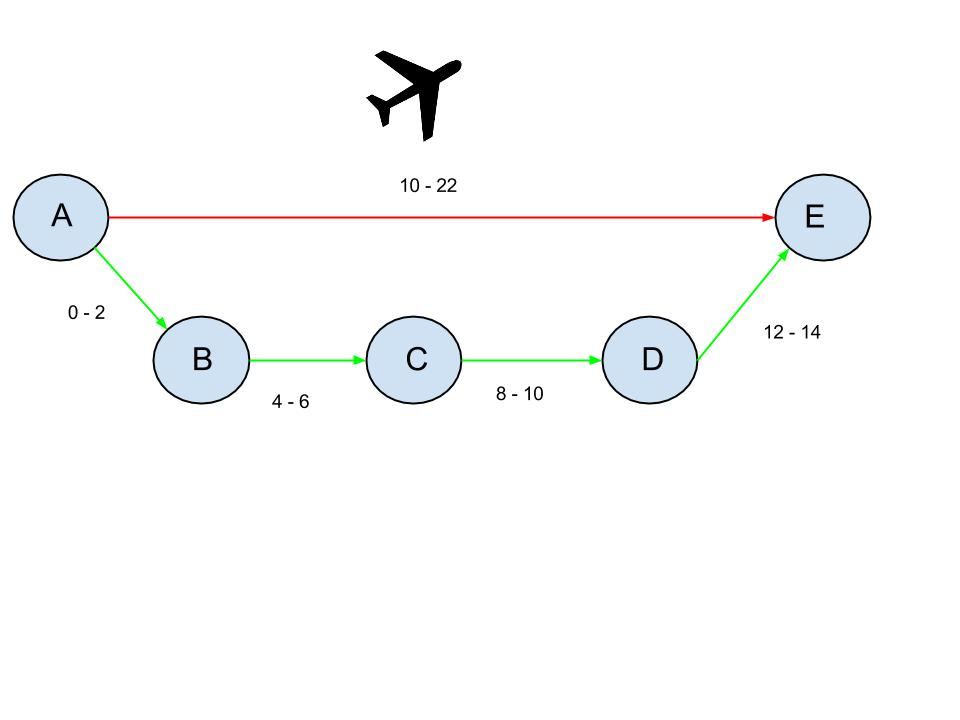
\includegraphics[scale=0.25]{imagenes/plane.jpg}
  %~ \end{center}
  %~ \caption{ejemplo de mejor vuelo.}
%~ \end{figure}
%~
%~
%~
%~ \newpage
%~ \subsection{Desarrollo de la idea y pseudocódigo.}
%~
%~ \vspace*{0.3cm}
%~
%~ Para resolverlo, se propone \textbf{ordenar} todos los \textbf{vuelos} disponibles
%~ \textbf{en base al horario de llegada, en forma ascendente}. Hecho esto, se recorre
%~ cada vuelo y se pregunta si es posible
%~
%~ \begin{enumerate}
  %~ \item llegar a la ciudad de origen \textbf{2 horas antes del horario de partida}.
%~
  %~ \item que la ciudad de partida de dicho vuelo es la ciudad de origen del cliente.
%~ \end{enumerate}
%~
%~ De valer alguno de estos ítems (\textbf{y si no hay otro vuelo que llegue antes
%~ a su destino}), se procede a marcar dicho vuelo como el primero en llegar y a
%~ su predecesor como el primero en llegar a la ciudad de origen. Caso contrario,
%~ el vuelo es ignorado.
%~
%~ Una vez recorridos todos, si existe algún vuelo que llegue al destino, existe
%~ solución, la cual se construye a partir de recorrer los vuelos predecesores.
%~ \textbf{Dicha cadena tiene como primer vuelo, aquel que parte desde la ciudad
%~ de origen del cliente.}
%~
%~
%~ \begin{codebox}
%~ \Procname{$\proc{planDeVuelo}(vuelos,origen,destino)$}
%~ \li \Comment $\id{vuelos}$ es un arreglo de tipo Vuelo, siendo Vuelo una
%~ \li \Comment estructura conformada por una ciudad origen, una ciudad destino,
%~ \li \Comment un horario de partida y otro de arribo.
%~ \li
%~ \li \Comment $\id{rutas}$ es un diccionario de ciudades en vuelos, en el cual,
%~ \li \Comment para cada ciudad, nos dice cual es el vuelo que llega antes.
%~ \li $\proc{ordenar}(vuelos)$
%~ \li $\id{rutas} \gets \emptyset$
%~ \li \While $\neg (\proc{vacio}(vuelos))$
%~ \li     \Do
            %~ $\id{vuelo} \gets \proc{primero}(vuelos)$
%~ \li         \If $\neg (\proc{existe}(\proc{destino}(vuelo),rutas)) \land
                %~ \proc{puedeTomar}(vuelo,rutas,origen)$
%~ \li             \Then
                    %~ $\id{rutas[\proc{destino}(vuelo)]} \gets vuelo$
                %~ \End
%~ \li         $\id{vuelos} \gets \id{vuelos} \setminus \{vuelo\}$
        %~ \End
%~ \li \If $\proc{existe}(destino,rutas)$
%~ \li     \Then
            %~ \Return $\proc{armarPila}(rutas,destino)$
%~ \li     \Else
%~ \li         \Return $\emptyset$
        %~ \End
%~ \end{codebox}
%~
%~
%~ \vspace*{0.3cm}
%~
%~
%~ \begin{codebox}
%~ \Procname{$\proc{puedeTomar}(vuelo,rutas,origen)$}
%~ \li \Return $\proc{origen}(vuelo) \isequal \id{origen} \lor
            %~ (\proc{existe}(\proc{origen}(vuelo),rutas) \land
             %~ \proc{llegada}(rutas[\proc{origen}(vuelo)]) \leq
             %~ \id{u} - 2)$
%~ \end{codebox}
%~
%~
%~ \vspace*{0.3cm}
%~
%~
%~ \begin{codebox}
%~ \Procname{$\proc{armarPila}(rutas,destino)$}
%~ \li $\id{lista} \gets \emptyset$
%~ \li \If $\proc{existe}(destino,rutas)$
%~ \li     \Then
            %~ $\id{vuelo} \gets \id{rutas[destino]}$
%~ \li         $\proc{agregarAdelante}(vuelo,lista)$
%~ \li         \While $\exists \hspace{0.07cm} \id{vuelo.predecesor}$
%~ \li             \Do
                   %~ $\id{vuelo} \gets \id{vuelo.predecesor}$
%~ \li                $\proc{agregarAdelante}(vuelo,lista)$
                %~ \End
%~ \li     \Else
%~ \li         \Return $\id{lista}$
        %~ \End
%~ \end{codebox}
%~
%~
%~
%~ \newpage
%~ \subsection{Análisis de complejidad.}
%~
%~ \vspace*{0.3cm}
%~
%~ Para el análisis de complejidad nos basaremos en el pseudocódigo de la función
%~ \textsc{planDeVuelo}, correspondiente al ítem \textbf{3.2}.
%~
%~ \begin{enumerate}
  %~ \item Todas las operaciones realizadas sobre el contenedor \verb|deque| de la
  %~ \textit{STL} (size, push_front, back y la creación de iteradores)
  %~ toman tiempo constante $O(1)$.
%~
  %~ \item De las operaciones realizadas sobre el contenedor \verb|map| de la
  %~ \textit{STL} (find, []) toman tiempo logarítmico $O(\log n)$ mientras que end y
  %~ la creación de iteradores, toman tiempo constante $O(1)$.
%~
  %~ \item Las operaciones realizadas sobre \verb|string| de la \textit{STL} toman
  %~ tiempo proporcional al tamaño del string. Pero asumimos que éstos están
  %~ acotados, por lo tanto las operaciones se realizan en tiempo constante
  %~ $O(1)$
%~
  %~ \item El algoritmo \verb|sort| de la \textit{STL} utilizado (línea \textcolor{red}{\textbf{completar!}})
  %~ para ordenar los aviones por horario de llegada, tiene complejidad $O(n \log n)$.
%~
  %~ \item Se implementó la función \verb|puedeTomar|, que dado un \verb|map|, un \verb|Vuelo| y
    %~ una ciudad, hace un \verb|find| sobre el \verb|map| y luego comparaciones y asignaciones.
    %~ Por lo tanto queda con una complejidad $O(\log n)$
%~
  %~ \item En la línea \textcolor{red}{\textbf{completar!}} se recorren todos los vuelos
    %~ y dentro se realizan 2 operaciones logarítmicas, quedando la complejidad del
    %~ ciclo como $O(n \log n)$
%~
  %~ \item Luego se genera la lista recorriendo los predecesores, como máximo pueden ser
    %~ todos los vuelos, es decir, $O(n)$
%~ \end{enumerate}
%~
%~
%~ Por lo tanto, la \textbf{complejidad total} del algoritmo implementado para este problema es
%~
%~ \begin{center}
  %~ $O(n \log n) + O(n \log n) + O(n) =$ \textit{\textbf{O(n log n)}}
%~ \end{center}
%~
%~ \textcolor{red}{\textbf{completar!}}
%~
%~
%~
%~ \newpage
\subsection{Experimentación y gráficos.}

\vspace*{0.3cm}

\subsubsection{Test 1 - benchmark aleatorio}

(ver \verb|info.1.v.dat|) \medskip

En este test, tenemos $k$ ciudades, con $k$ inicializado en 100 e incrementándose de a 1000, hasta alcanzar 20000 y $n$ vuelos, inicializados en 1000, incrementándose de a 1000, hasta alcanzar 200000.

Para cada instancia se toma el \textbf{valor mínimo} de microsegundos luego de
\textbf{25 corridas}.

\vspace*{0.5cm}

\begin{figure}[h]
  \begin{center}
    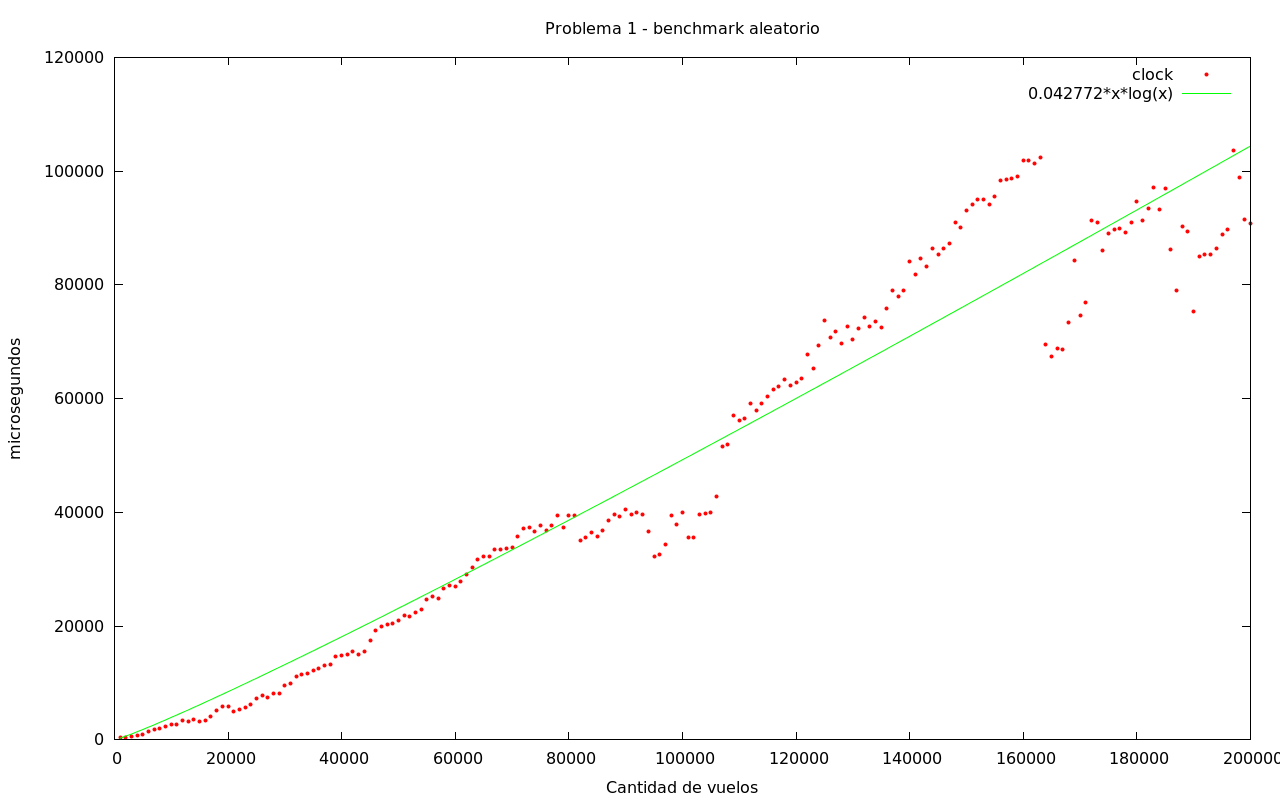
\includegraphics[scale=0.35]{imagenes/grafico-1-v.png}
  \end{center}
\end{figure}

\vspace*{0.5cm}

En este gráfico vemos que, si bien no parece comportarse como una curva del orden $n*\log n$, al dividir la misma por $\log k + \log n$, obtenemos el siguiente gráfico:

\vspace*{0.5cm}

\begin{figure}[h]
  \begin{center}
    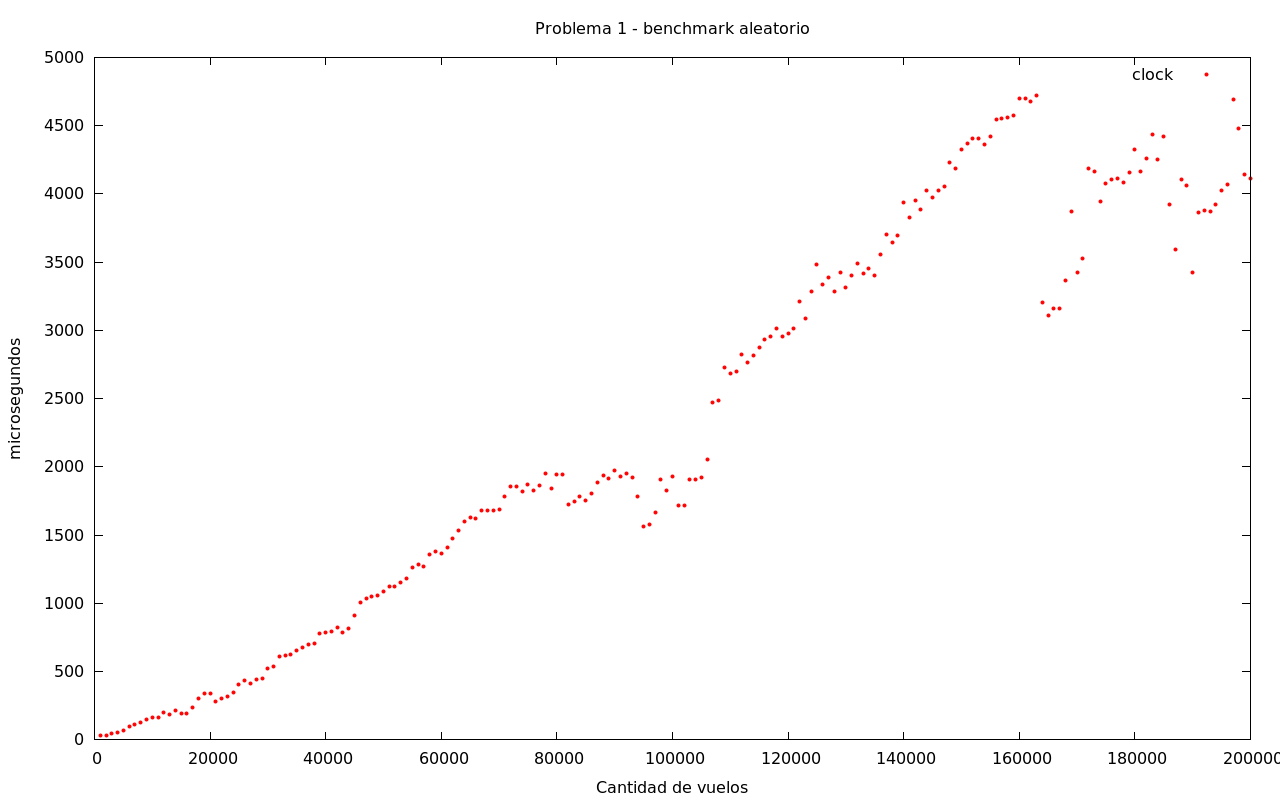
\includegraphics[scale=0.35]{imagenes/grafico-1-v-ajustado.png}
  \end{center}
\end{figure}

\vspace*{0.5cm}

Ahora vemos que la nueva curva queda lineal, porque, pese que en el análisis téórico de la complejidad del algoritmo determinamos que era del orden $O(n*\log n)$, esta en realidad se trata de una cota superior que nos abstrae del detalle de la cantidad de ciudades, pues sabemos que esta cantidad vale, a lo sumo $2*n$, pues hay 2 ciudades por vuelo y en el peor de los casos, todas las ciudades son distintas. Por lo tanto, la complejidad exacta del algoritmo sería $O(vuelos*\log(vuelos) + vuelos*\log(ciudades))$. Dado que               $ciudades \leq 2*vuelos$, el algoritmo termina perteneciendo al orden $O(n*\log n)$.
